\section{Actividad 01: Importación de datos usando el Wizard - Sql Managment} 

1. Crearemos una base de datos llamada BDTEST\\
	\begin{center}
	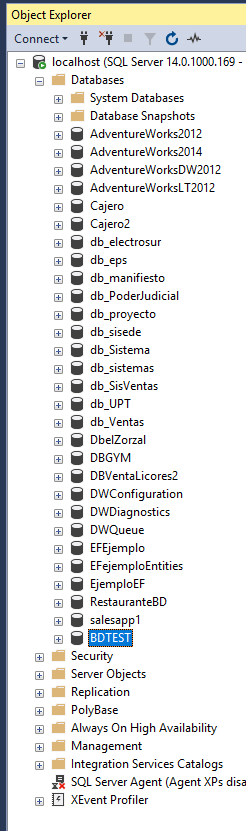
\includegraphics[width=7cm,height=21cm]{./Imagenes/img1}
	\end{center}	


2.  Importamos la  base de datos desde AdventureWorks.\\
	\begin{center}
	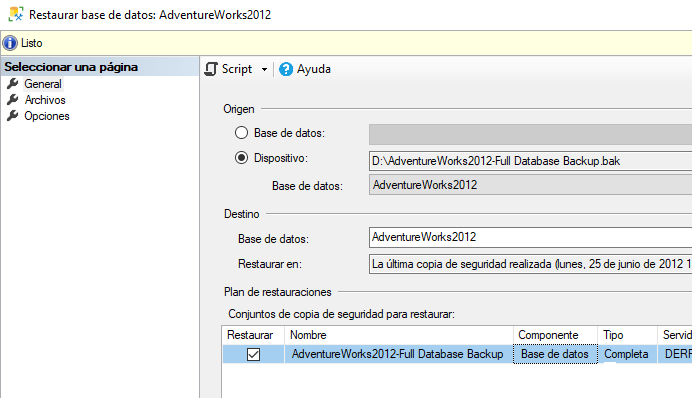
\includegraphics[width=11cm]{./Imagenes/img2}
	\end{center}	
\pagebreak
3. Escribir el Servidor y seleccionar la base de datos\\
	\begin{center}
	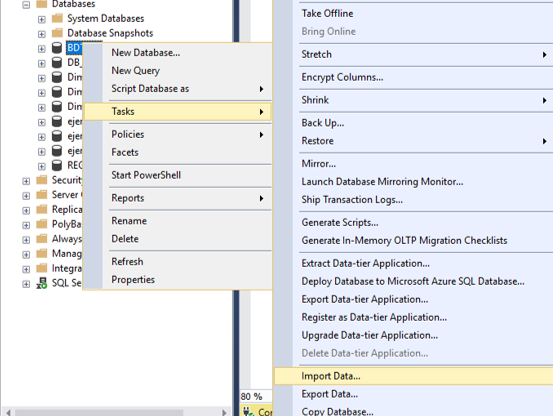
\includegraphics[width=13cm]{./Imagenes/img3}
	\end{center}	

4. Data Source: La base de donde vamos a importar 
	\begin{center}
	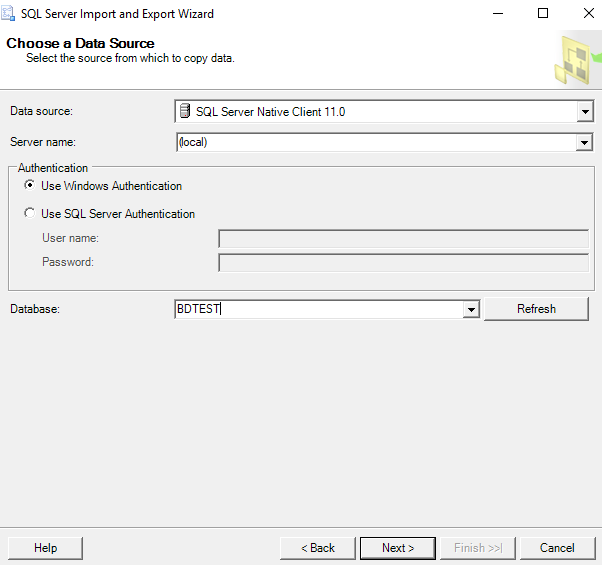
\includegraphics[width=12cm]{./Imagenes/img4}
	\end{center}	
5. Destination: La Base donde vamos a cargar los datos\\
	\begin{center}
	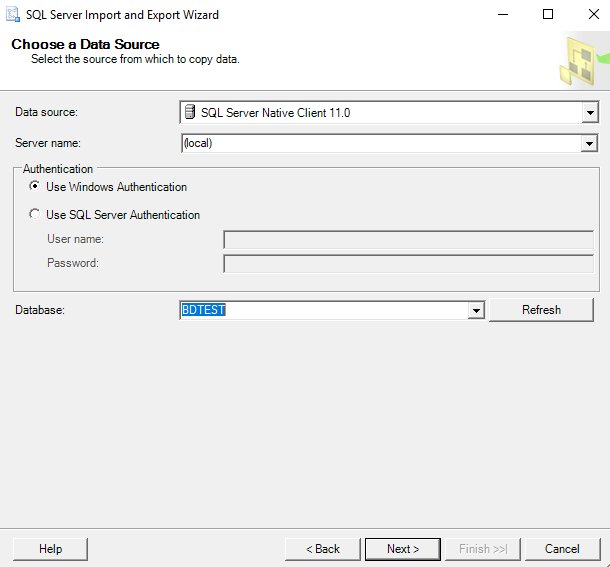
\includegraphics[width=12cm]{./Imagenes/img5}
	\end{center}	
6. Especificar si se realizará copia o consulta, en este caso elejimos copia.\\
	\begin{center}
	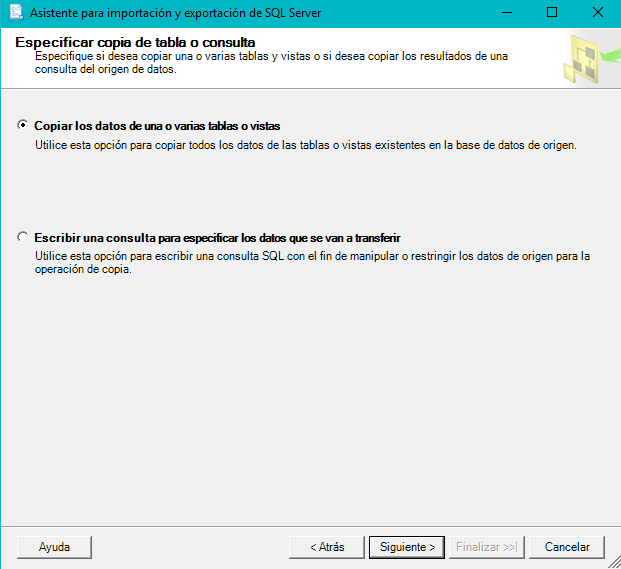
\includegraphics[width=11cm]{./Imagenes/img6}
	\end{center}	
7. Seleccionamos las tablas HumanResources y Person
	\begin{center}
	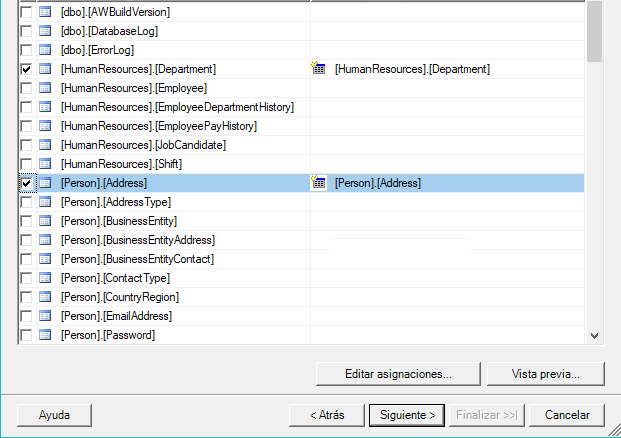
\includegraphics[width=11cm]{./Imagenes/img7}
	\end{center}	
8. Guardamos y ejecutamos.
	\begin{center}
	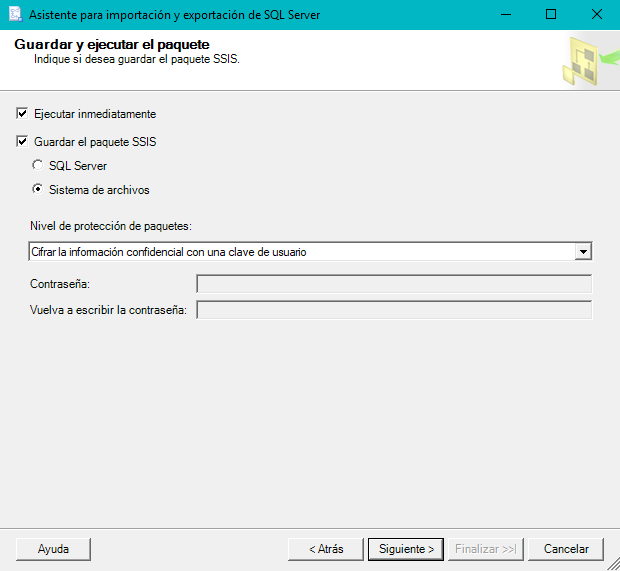
\includegraphics[width=11cm]{./Imagenes/img8}
	\end{center}	
	\begin{center}
	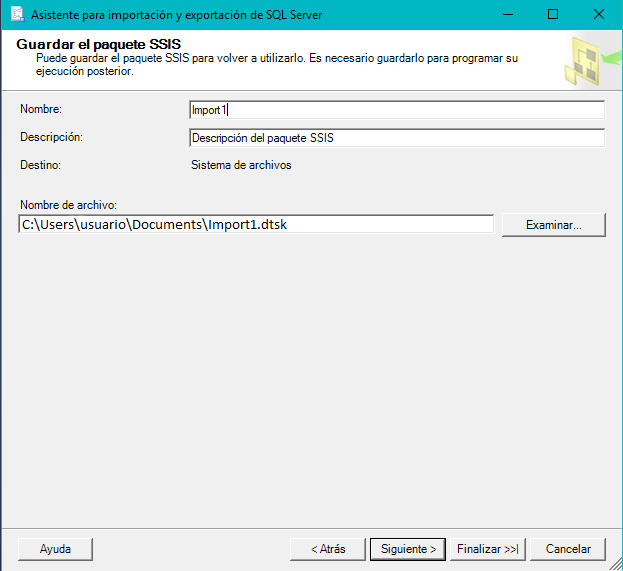
\includegraphics[width=11cm]{./Imagenes/img9}
	\end{center}	
	\begin{center}
	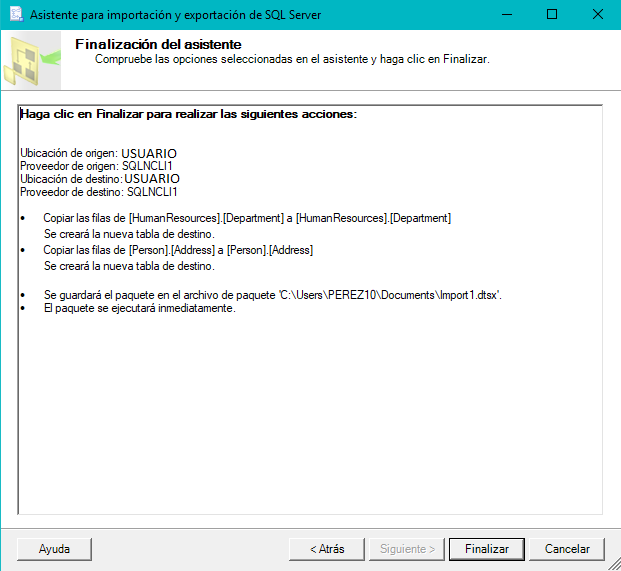
\includegraphics[width=11cm]{./Imagenes/img10}
	\end{center}	

	\begin{center}
	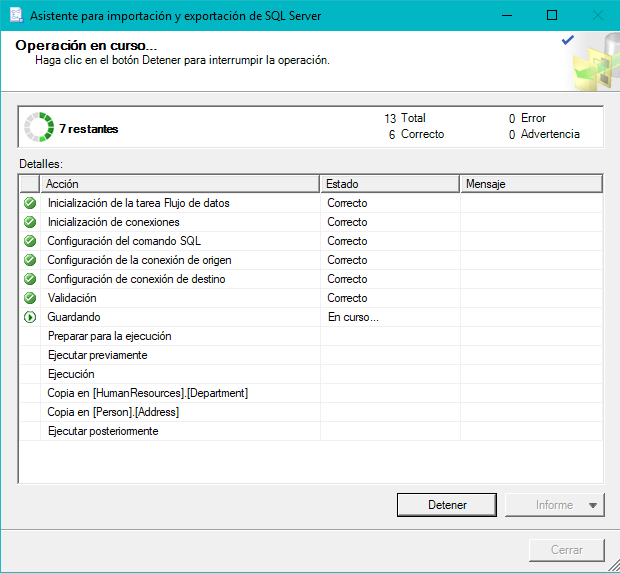
\includegraphics[width=11cm]{./Imagenes/img11}
	\end{center}	
5. Se observa que se realizó correctamente  la ejecución\\
	\begin{center}
	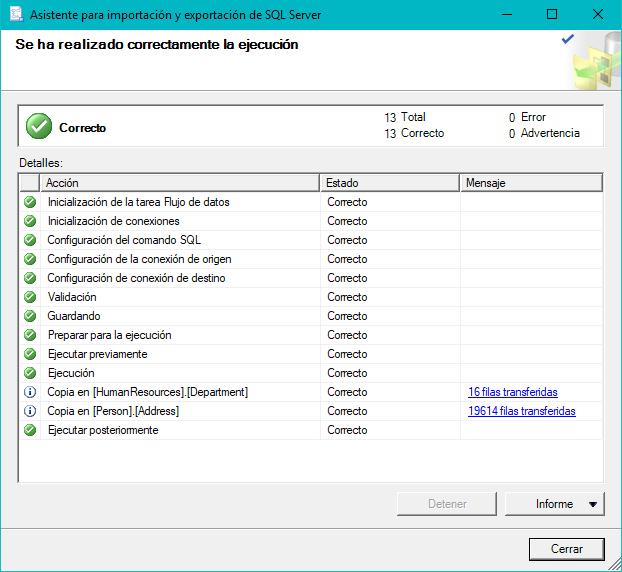
\includegraphics[width=11cm]{./Imagenes/img12}
	\end{center}	